\section{Results}

Descriptive statistics and correlations among study variables are shown in Table~\ref{tab:correlations}. Overall, both identification with educational value (IEV) and academic prosocial behavior (APB) significantly declined from Time 1 to Time 2. As illustrated in the latent change score models (Figure~\ref{fig:LCM_simple}), IEV showed a significant negative change ($\beta = -0.334, p < .001$), and APB also declined ($\beta = -0.514, p < .001$). Moreover, changes in IEV and APB were positively correlated, suggesting that students who showed stronger declines in one domain tended to show stronger declines in the other.  

The full structural model (Figure~\ref{fig:LCM_full}) further indicated that perceived economic inequality (PEI) at baseline predicted greater decreases in IEV over time, but was not significantly related to changes in APB. Declines in IEV were associated with decreases in life satisfaction, while declines in APB were associated with decreases in positive affect and increases in negative affect. These findings provide partial support for our hypothesis that perceived economic inequality would predict reductions in IEV and APB, and confirm that both declines are linked with reduced well-being.  

\begin{figure}[htbp]
\centering
\begin{tikzpicture}[node distance=2.8cm, >=Stealth, every node/.style={font=\small}]

  \tikzstyle{state}=[ellipse, draw, minimum width=24mm, minimum height=10mm, align=center]

  \node[state]                          (IEV1)   {IEV [T1]};
  \node[state, right=4.2cm of IEV1]     (IEV2)   {IEV [T2]};
  \node[state, above right=1.4cm and 2.1cm of IEV1] (dIEV) {$\Delta$ IEV};

  \draw[->] (IEV1) -- node[below] {1} (IEV2);
  \draw[->] (dIEV) -- node[above] {1} (IEV2);
  \draw[->, bend left=18] (IEV1) to node[above left] {$-0.334^{***}$} (dIEV);

  \node at ($(IEV1)!0.5!(IEV2)+(0,-1.3)$) {(a)};

  \node[state, below=3.8cm of IEV1]          (APB1)   {APB [T1]};
  \node[state, right=4.2cm of APB1]          (APB2)   {APB [T2]};
  \node[state, above right=1.4cm and 2.1cm of APB1] (dAPB) {$\Delta$ APB};

  \draw[->] (APB1) -- node[below] {1} (APB2);
  \draw[->] (dAPB) -- node[above] {1} (APB2);
  \draw[->, bend left=18] (APB1) to node[above left] {$-0.514^{***}$} (dAPB);

  \node at ($(APB1)!0.5!(APB2)+(0,-1.3)$) {(b)};
\end{tikzpicture}
\caption{Latent change score models for IEV (a) and APB (b).}
\label{fig:LCM_simple}
\end{figure}


\begin{figure}[htbp]
\centering
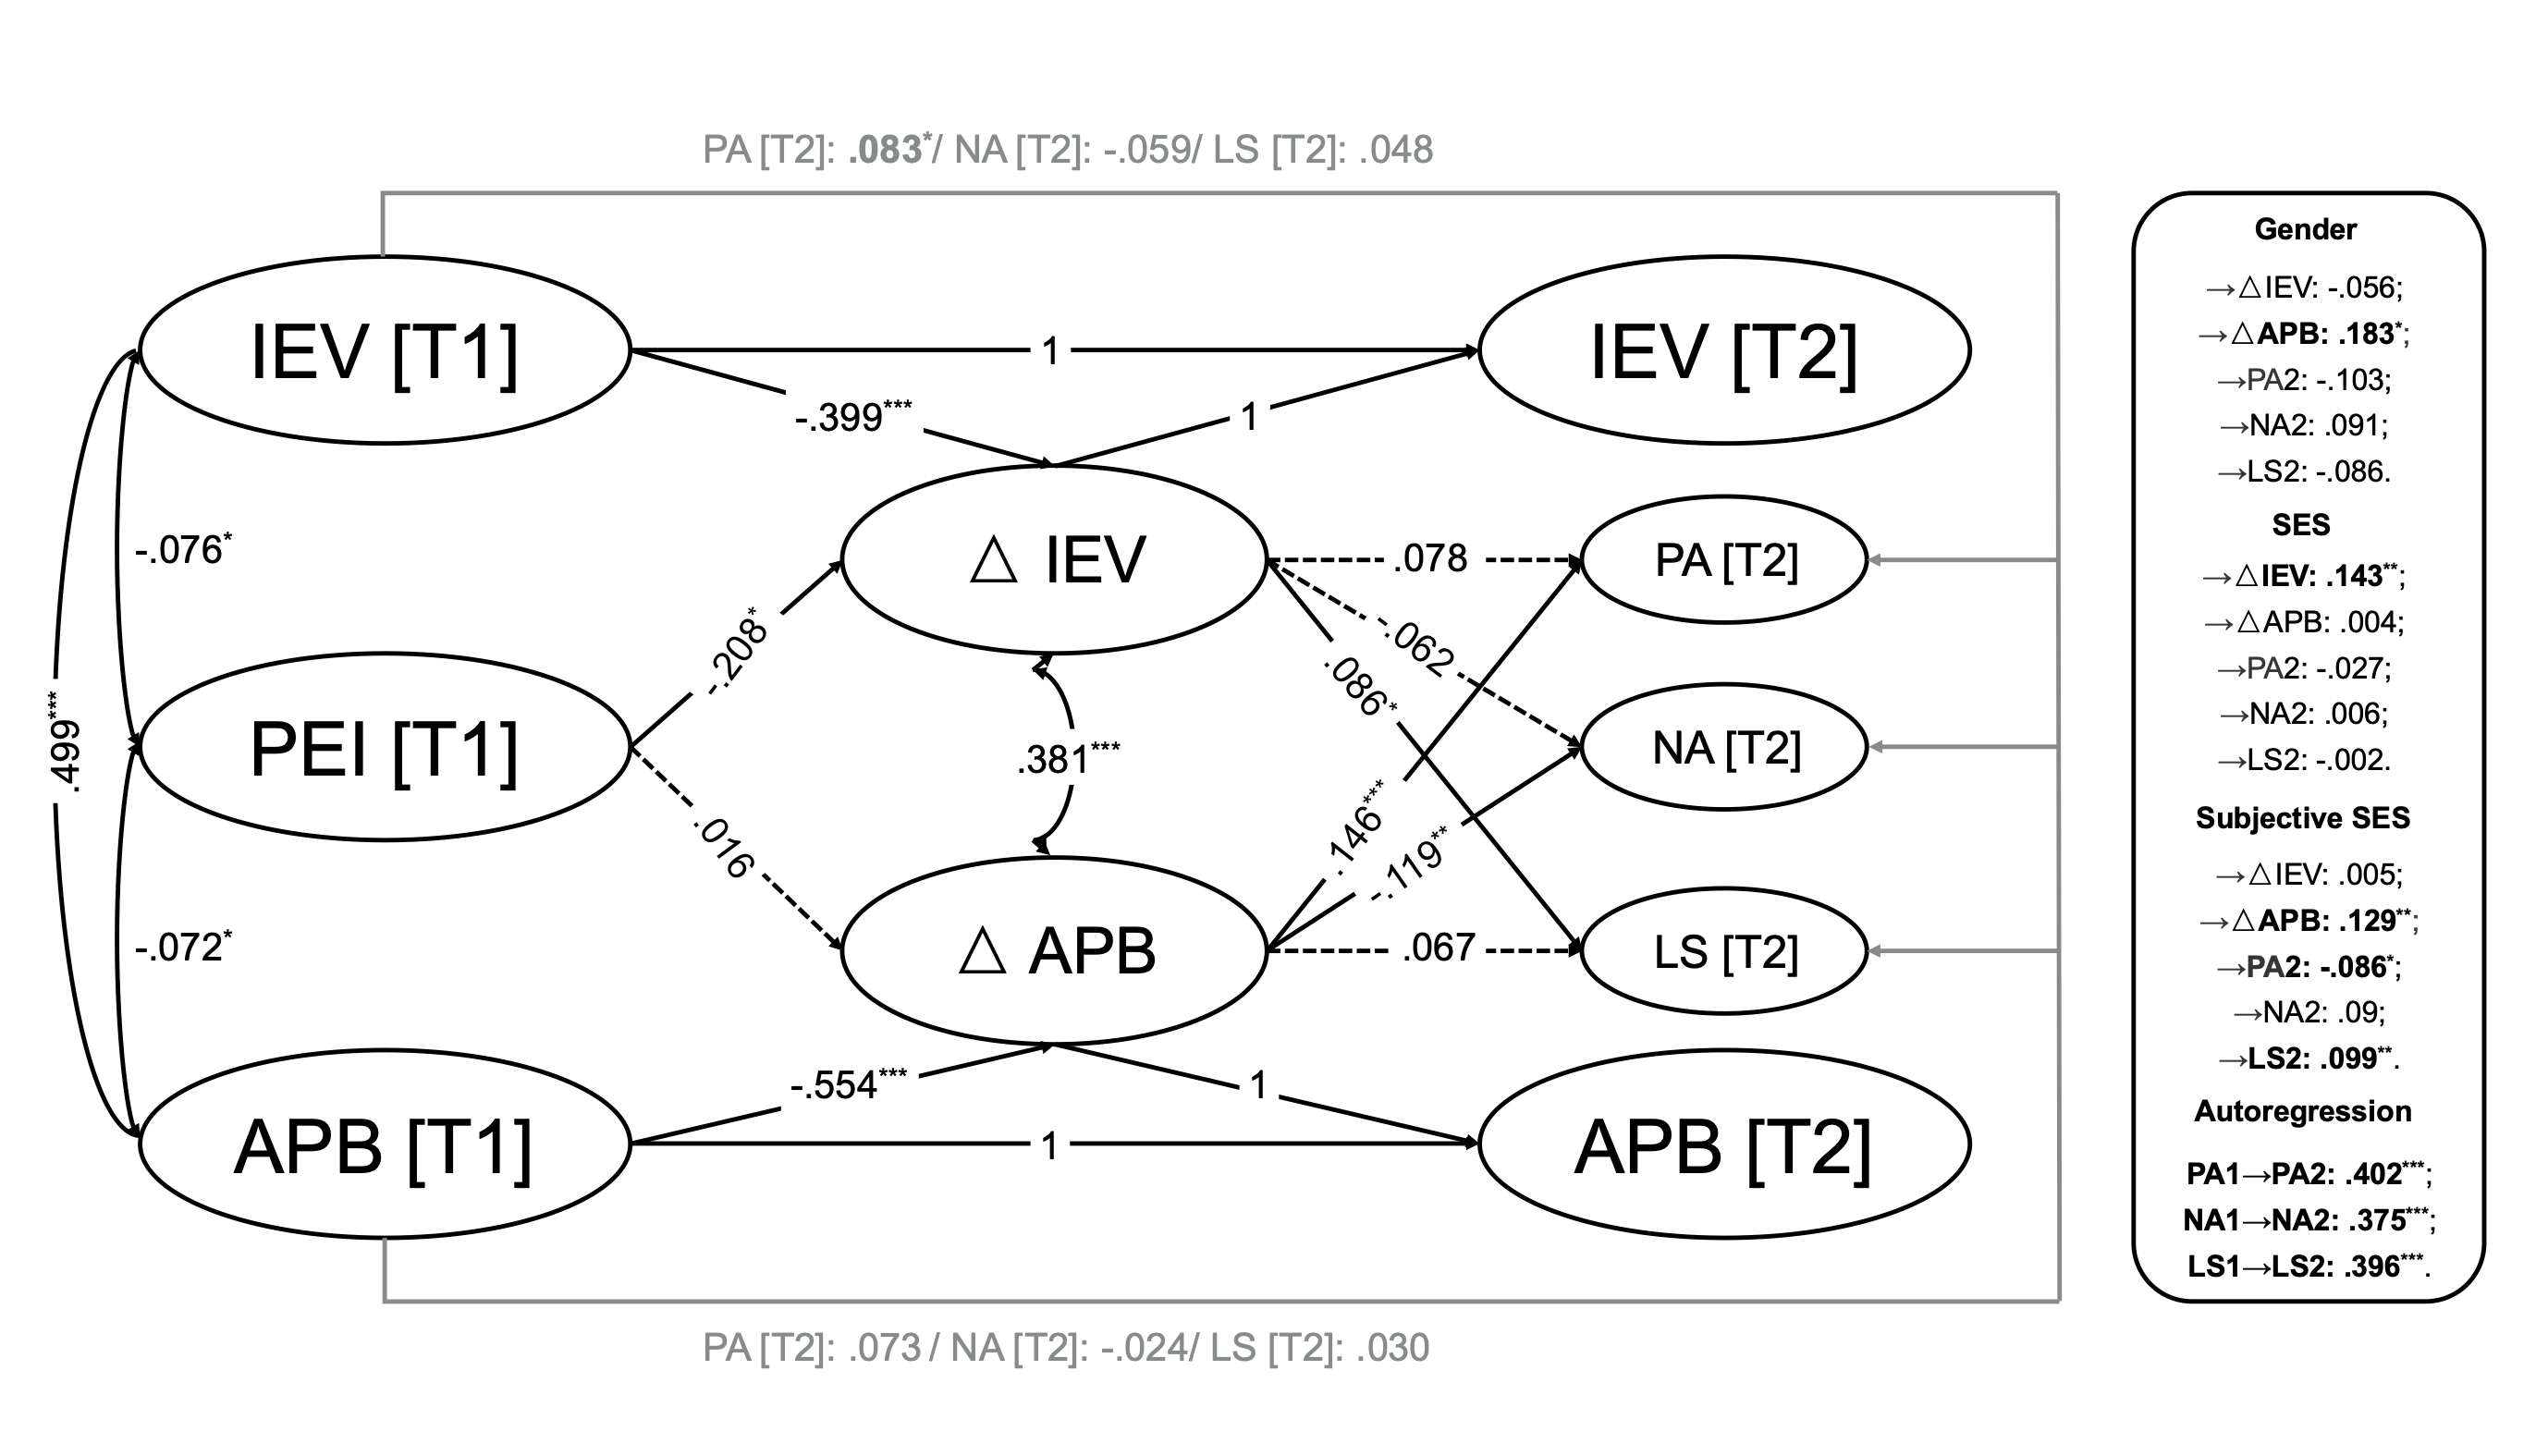
\includegraphics[width=0.9\textwidth]{20250829_Figure3.png}
\caption{Full structural model including perceived economic inequality (PEI), identification with educational value (IEV), academic prosocial behavior (APB), and well-being indicators.}
\label{fig:LCM_full}
\end{figure}

\begin{sidewaystable}[htbp]
\centering
\caption{Descriptive statistics and correlations among study variables}
\label{tab:correlations}
\begin{threeparttable}
\begin{tabular}{lcccccccccccccc}
\toprule
Variable & $M$ & $SD$ & ICC & 1 & 2 & 3 & 4 & 5 & 6 & 7 & 8 & 9 & 10 & 11 \\
\midrule
1. T1 PEI        & 2.73 & 1.494 & \textbf{.108} & -- \\
2. T1 IEV        & 5.73 & 1.245 & .018  & -.103* & -- \\
3. T2 IEV        & 5.35 & 1.476 & $<$.001 & -.143*** & .575*** & -- \\
4. T1 APB        & 5.18 & 1.643 & .015  & -.085 & .399*** & .208*** & -- \\
5. T2 APB        & 4.95 & 1.757 & .025  & -.043 & .202*** & .390*** & .511*** & -- \\
6. T1 PA         & 3.72 & 1.083 & .011  & -.179*** & .205*** & .102* & .324*** & .260*** & -- \\
7. T2 PA         & 3.65 & 1.007 & .017  & -.151** & .160** & .215*** & .161*** & .295*** & .515*** & -- \\
8. T1 NA         & 2.61 & 1.058 & .021  & .166** & -.104 & -.086 & -.014 & -.115* & -.405*** & -.330*** & -- \\
9. T2 NA         & 2.49 & .932  & .046  & .229*** & -.092 & -.216*** & .042 & -.188*** & -.316*** & -.452*** & .568*** & -- \\
10. T1 LS        & 3.34 & 1.183 & .002  & -.087 & .201*** & -.030 & .224*** & .136*** & .341*** & .282*** & -.265*** & -.092 & -- \\
11. T2 LS        & 3.36 & 1.083 & \textbf{.077} & -.109* & .116* & .158*** & .114* & .201*** & .290*** & .506*** & -.235*** & -.423*** & .484*** & -- \\
\bottomrule
\end{tabular}
\begin{tablenotes}
\footnotesize
\item \textit{Note}. $N = 634$. PEI = Perceived Economic Inequality; IEV = Identification with Educational Values; APB = Academic Prosocial Behavior; PA = Positive Affect; NA = Negative Affect; LS = Life Satisfaction. 
\item * $p < .05$. ** $p < .01$. *** $p < .001$.
\end{tablenotes}
\end{threeparttable}
\end{sidewaystable}

